\documentclass{article}
\usepackage[en]{homework}
\usepackage{tikz}

\config{Physics-1}{2026 Fall}{1}

\begin{document}

\begin{problem}
Fun with estimating:

In humans, oxygen and carbon dioxide are exchanged in the blood within many small sacs called alveoli in the lungs. Alveoli provide a large surface area for gas exchange. Recent careful measurements show that the total number of alveoli in a typical pair of lungs is about $480 \times 10^{6}$ and that the average volume of a single alveolus is $4.2 \times 10^{6}\,\mu\mathrm{m}^{3}$. ($\mu\mathrm{m}=10^{-6}\,\mathrm{m}$)

\begin{enumerate}
  \item[a)] Estimate the total volume of the gas-exchanging region of the lungs?
  \item[b)] If we assume that alveoli are spherical, what is the diameter of a typical alveolus?
\end{enumerate}
\end{problem}

\begin{solution}
	a) The total number of the gas-exchanging region of a pair of lungs is approxmately 
	\[ (480 \times 10^6) \times (4.2 \times 10^{6} \mathrm{\mu m}^3) \approx 2 \times 10^{15} \mathrm{\mu m}^{3} = 2 \,\mathrm{L}. \]

	b) Suppoes the radius of a single alveolus is $r$, then 
	\[ \frac{4}{3}\pi r^3 = 4.2 \times 10^{6} \mathrm{\mu m} 
	\implies r \approx 100 \mathrm{\mu m}. \]
	So the typical diameter of an alveolus is $2r \approx 200 \mathrm{\mu m}$.
\end{solution}



\begin{problem}
Linear deceleration problem.

A neutron travels at a speed of $1.4 \times 10^{7}\,\mathrm{m/s}$. Nuclear forces are of very short range, being essentially zero outside a nucleus but very strong inside. If the neutron is captured and brought to rest by a nucleus whose diameter is $1.0 \times 10^{-14}\,\mathrm{m}$, what is the minimum magnitude of the force, presumed to be constant, that acts on this neutron?

The neutron's mass is $1.67 \times 10^{-27}\,\mathrm{kg}$.
\end{problem}

\begin{solution}
	The minimum deceleration $a>0$ of the neturon is given by
	\[ 2ad = v_0^2 \implies a = \frac{v_0^2}{2d}, \]
	where $v_0$ is the initial speed of the neutron, and $d$ is the diameter of the nucleus.

	Then the minimum force applied to the neturon is 
	\[ F = ma = \frac{mv_0^2}{2d}. \]
	Substitute the value of $m, v_0, d$, we got $F \approx 16.37\,\mathrm{N}$.
\end{solution}



\begin{problem}
Consider a pendulum made of a stick of mass $M$ and length $L$. You hold the pendulum so that it makes the initial angle $\theta$, and let it go. It starts swinging back and forth under the influence of gravity; let $T$ be the period of this motion.

By considering the dimensions of the quantities, try to find the form of $T$ as a function of $M$, $L$, $\theta$ and $g$. (i.e. there is a combination of $M,L,g,\theta$ so that they together has the dimension of time. This is a candidate for the dependence of $T$ on $M$, $L$ and $g$ etc).

The answer you just found should involve an undetermined function $f(\theta)$. What can you say about this function based on symmetry?
\end{problem}

\begin{solution}
	We use $\mathrm{T,M,L}$ to represent the dimension of time, mass and length. Note that
	\[ [T] = \mathrm{T}, \quad [M] = \mathrm{M}, \quad [L] = \mathrm{L}, \quad [\theta] = 1, \quad [g] = \mathrm{LT^{-2}}. \]
	So the only way to construct $T$ from $L,M,\theta$ is
	\[ T = \sqrt{\frac{l}{g}}f(\theta), \]
	where $f(\theta)$ is an undetermined function.

	Since the transformation $\theta \to -\theta$ represents the spatial reflection w.r.t the symmetry axis of the pendulum, which does not change the period of the pendulum, we have $f(-\theta) = f(\theta)$.
\end{solution}



\begin{problem}
\begin{enumerate}
  \item[a)] All of the surfaces in the setup below are frictionless. You push on the large block and give it an acceleration $a$. For what value of $a$ is there no relative motion among the masses?

  \begin{center}
    \begin{tikzpicture}[scale=0.85, line width=0.6pt]
      \fill[gray!30] (0,-0.25) rectangle (4.5,0);
      \draw (0,0) -- (4.5,0);
      \draw[fill=shadecolor] (0.45,0) rectangle (3.1,2.65);
      \draw[fill=shadecolor] (1.1,2.65) rectangle (2.3,3.55);
      \draw[fill=shadecolor] (3.1,0.85) rectangle (3.9,2.1);
      \draw (2.3,3.08) -- (3.38,3.08);
      \draw (3.38,2.9) circle (0.18);
      \draw (3.56,2.9) -- (3.56,2.1);
      \node at (1.75,3.1) {$m_1$};
      \node at (1.77,1.55) {$M$};
      \node at (3.5,1.47) {$m_2$};
      \draw[->] (1.15,0.75) -- (2.2,0.75);
      \node[above] at (1.65,0.75) {$a$};
    \end{tikzpicture}
  \end{center}

  \item[b)] Now assume that the string is not massless. It has mass per unit length $\rho$. Assume that the string has total length $L$ and the horizontal segment has length $x$. How does that change the answer in a)?
\end{enumerate}
\end{problem}

\begin{solution}
	(a) Consider the problem in the non-inertial reference frame, in which the mass $M$ dose not move. Then there will exist a inertial force applied on the mass $m_1$ with magnitude $am_1$ and towards left. The inertial force is equal to the gravity of $m_2$ due to the relative stationary among the masses. Hence we have
	\[ am_1 = gm_2 \implies a = \frac{gm_2}{m_1}. \]

	(b) The argument above is still valid, but we need to consider the inertial force and the gravity applied on the string:
	\[ a(m_1+x\rho) = g(m_2 + (L-x)\rho) \implies a = \frac{m_2 + (L-x)\rho}{m_1 + x\rho} g. \]
\end{solution}



\begin{problem}
Consider the $N$ pulleys system. A string passes over each pulley, with one end attached to a mass $m$ and the other end attached to another pulley. For the $N$-th pulley, the other end of the string is attached to a mass $m$. All the pulleys and strings are massless. The masses are held fixed and then simultaneously released.

\begin{enumerate}
  \item[a)] Let $N=2$, calculate the accelerations of all the masses?
  \item[b)] Let $N=3$, calculate the accelerations of all the masses?
  \item[c)] Let $N$ goes to infinity, what is the acceleration of the top mass?
\end{enumerate}

\begin{center}
  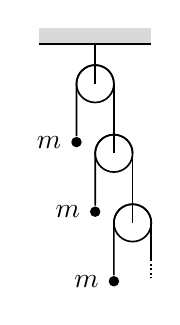
\begin{tikzpicture}[scale=0.95, line width=0.6pt]
    \fill[gray!30] (0,4.78) rectangle (1.5,5.0);
    \draw (0,4.78) -- (1.5,4.78);
    \draw (0.75,4.78) -- (0.75,4.25);
    \draw (0.75,4.25) circle (0.25);
    \draw (0.5,3.55) -- (0.5,4.25) arc[start angle=180,end angle=0,radius=0.25];
    \draw (1.0,4.25) -- (1.0,3.32);
    \fill (0.5,3.47) circle (0.07);
    \node[left] at (0.43,3.47) {$m$};
    \draw (1.0,3.32) circle (0.25);
    \draw (0.75,2.62) -- (0.75,3.32) arc[start angle=180,end angle=0,radius=0.25];
    \draw (1.25,3.32) -- (1.25,2.39);
    \fill (0.75,2.54) circle (0.07);
    \node[left] at (0.68,2.54) {$m$};
    \draw (1.25,2.39) circle (0.25);
    \draw (1.0,1.69) -- (1.0,2.39) arc[start angle=180,end angle=0,radius=0.25];
    \draw (1.5,2.39) -- (1.5,1.9);
    \draw[densely dotted] (1.5,1.9) -- (1.5,1.65);
    \fill (1.0,1.61) circle (0.07);
    \node[left] at (0.93,1.61) {$m$};
  \end{tikzpicture}
\end{center}
\end{problem}

\begin{solution}
	We consider the general case in which there are $N$ pulleys. Noting that all the pulleys and strings are massless, so we can denote the tension of each string and the acceleration of each mass as shown in the following figure.
	\begin{figure}[H]
		\centering
		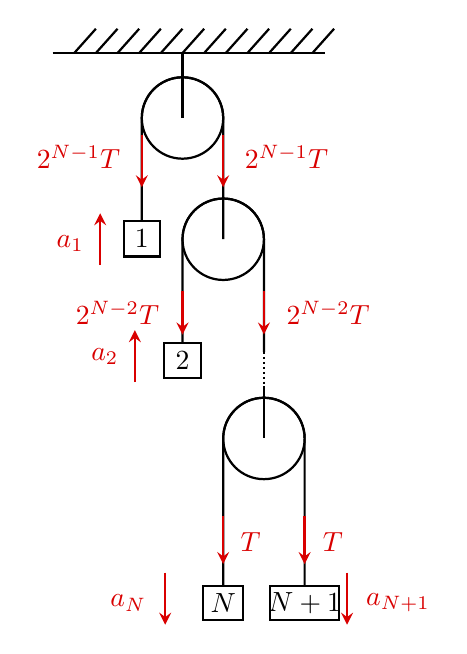
\begin{tikzpicture}[scale=1.1, line width=0.8pt, >=stealth]
			% Ceiling and support for the fixed pulley.
			\draw (0.5,6.9) -- (3.65,6.9);
			\foreach \x in {0.75,1.0,...,3.5} {
				\draw (\x,6.9) -- ++(0.25,0.28);
			}
			\draw (2,6.9) -- (2,6.15);
			\draw (2,6.15) circle (0.47);

			% The first string supports mass 1 and the second pulley.
			\draw (1.53,4.96) -- (1.53,6.15)
				arc[start angle=180,end angle=0,radius=0.47] -- (2.47,4.75);
			\draw (1.32,4.55) rectangle (1.74,4.96);
			\node at (1.53,4.755) {$1$};
			\draw (2.47,4.75) circle (0.47);

			% The second string supports mass 2 and the last pulley.
			\draw (2,3.55) -- (2,4.75)
				arc[start angle=180,end angle=0,radius=0.47] -- (2.94,3.45);
			\draw[densely dotted] (2.94,3.45) -- (2.94,3.05);
			\draw (2.94,3.05) -- (2.94,2.45);
			\draw (1.79,3.15) rectangle (2.21,3.55);
			\node at (2,3.35) {$2$};
			\draw (2.94,2.45) circle (0.47);

			% The final string supports masses N and N+1.
			\draw (2.47,0.75) -- (2.47,2.45)
				arc[start angle=180,end angle=0,radius=0.47] -- (3.41,0.75);
			\draw (2.24,0.35) rectangle (2.7,0.75);
			\node at (2.47,0.55) {$N$};
			\draw (3.01,0.35) rectangle (3.81,0.75);
			\node at (3.41,0.55) {$N+1$};

			% Tensions and accelerations shown in the supplied diagram.
			\begin{scope}[red!85!black, line width=0.9pt]
				\draw[->] (1.53,5.95) -- (1.53,5.35);
				\draw[->] (2.47,5.95) -- (2.47,5.35);
				\node[left] at (1.4,5.7) {$2^{N-1}T$};
				\node[right] at (2.6,5.7) {$2^{N-1}T$};
				\draw[->] (1.05,4.45) -- (1.05,5.05);
				\node[left] at (0.98,4.7) {$a_1$};

				\draw[->] (2,4.15) -- (2,3.65);
				\draw[->] (2.94,4.15) -- (2.94,3.65);
				\node[left] at (1.85,3.9) {$2^{N-2}T$};
				\node[right] at (3.08,3.9) {$2^{N-2}T$};
				\draw[->] (1.45,3.1) -- (1.45,3.7);
				\node[left] at (1.38,3.4) {$a_2$};

				\draw[->] (2.47,1.55) -- (2.47,1.0);
				\draw[->] (3.41,1.55) -- (3.41,1.0);
				\node[right] at (2.55,1.25) {$T$};
				\node[right] at (3.5,1.25) {$T$};
				\draw[->] (1.8,0.9) -- (1.8,0.3);
				\node[left] at (1.7,0.55) {$a_N$};
				\draw[->] (3.9,0.9) -- (3.9,0.3);
				\node[right] at (4.0,0.55) {$a_{N+1}$};
			\end{scope}
		\end{tikzpicture}
	\end{figure}
	For each mass, according to the Newton's Second Law and the geometric relation, we have
	\[ \begin{cases}
		mg - 2^{N-k}T = ma_k & (1\le k\le N) \\
		a_{N+1} = a_N \\
		\sum_{k=1}^{N}2^{N-k}a_k+a_{N+1} = 0.
	\end{cases} \]
	Solving this linear equation, we got
	\[ a_k = \left( 1 - \frac{3\cdot 2^{2N-k-1}}{2^{2N-1}+1} \right)g\ (1\le k\le N),\quad a_{N+1} = a_N. \]
	
	a) For $N=2$, we have
	\[ a_1 = -g/3, \quad a_2 = a_3 = g/3; \]

	b) For $N=3$, 
	\[ a_1 = -\frac{5}{11}g, \quad a_2 = \frac{3}{11}g, \quad a_3 = a_4 = \frac{7}{11}g. \]

	c) For $N\to\infty$, the acceleration of top mass approxs to 
	\[ a_1 = \lim_{N\to\infty}\left( 1-\frac{3\cdot2^{2N-2}}{2^{2N-1} + 1} \right)g = -g/2. \]
\end{solution}



\begin{problem}[optional]
A spring with spring constant $k$, natural length $L$ and total mass $M$ is initially at rest.

\begin{enumerate}
  \item[a)] A spring has spring constant $k$. If it is cut in half, what is the spring constant of each of the resulting shorter springs?
  \item[b)] Consider pulling the spring at its right end with a force $F$ towards the right. The left end is not fixed to anything and the entire system moves forward. How long would the spring become?
\end{enumerate}
\end{problem}

\begin{solution}
	a) Consider pulling the spring with force $k \Delta x$. Then each of the half of the complete spring become $k \Delta x/2$ longer than before, while the tension of the two springs are also $k\Delta x$. So the spring constant of two new spring is
	\[ k' = \frac{k\Delta x}{k\Delta x/2} = 2k. \]

	b) The overall acceleration of the spring is
	\[ a = F/M. \]
	Select the non-inertial reference frame in which the spring is constant. Equally slice the spring into $N$ piece. Because the existance of acceleration of the reference frame, the tension between $n$-th slice and the $(n+1)$-th slice of the spring is $an(M/N) = nF/N$, where the $1$-th slice refers to the most left slice of the spring. Then the amount of the elongation of $n$-th spring is
	\[ \Delta x_n = \frac{nF/N}{kN} = \frac{n}{N^2} \frac{F}{k}. \]

	The total amount of the elongation is
	\[ \Delta x = \sum_{n=1}^{N}\Delta x_n = \frac{N+1}{2N} \frac{F}{k}. \]

	Let $N \to \infty$, we got
	\[ \Delta x = \frac{F}{2k}. \]
\end{solution}



\end{document}
